\documentclass[12pt]{article} % Establece el tamaño de fuente en 12pt
% Paquetes para configurar el idioma, codificación y fuente
\usepackage[utf8]{inputenc} % Codificación de entrada
\usepackage[spanish]{babel}
\usepackage[T1]{fontenc} % Codificación de fuente
%\usepackage[spanish]{babel} % Idioma español
\usepackage{mathptmx}
\usepackage{amsmath}
\usepackage{graphicx}
\usepackage{subcaption}
\usepackage{imakeidx}
\renewcommand{\contentsname}{Índice}
\usepackage[letterpaper, margin=2.5cm, top=3.5cm, bottom=2.5cm]{geometry} % Configura el tamaño de papel y márgenes
\makeindex[columns=3, title=Alphabetical Index, intoc]
\usepackage{setspace} % Para configurar el espaciado entre líneas
\usepackage{booktabs} % Para las líneas de las tablas
\doublespacing % Establece un espaciado doble
\usepackage{siunitx} % Para alinear las cifras decimales

\sisetup{
 round-mode          = places, % Redondea los números
  round-precision     = 2, % a 1 cifra decimal
    output-decimal-marker = {.}, % Usa puntos para los decimales
  group-separator={,}, % Usa comas como separadores de miles
  group-minimum-digits    = 4 % Agrupa dígitos por miles a partir de 4 cifras
}

\usepackage{caption}
\usepackage{hyperref}
\usepackage{float}
\usepackage{listings}
\usepackage{amssymb}
\usepackage{amsfonts}
\usepackage{mdframed}
\usepackage{pgfplots}
\pgfplotsset{compat=1.15}
\usepackage{mathrsfs}
\usetikzlibrary{arrows}
\usepackage{xcolor}
\lstset{
    language=Python,
    basicstyle=\ttfamily\footnotesize,
    backgroundcolor=\color{gray!10}, % Color de fondo
    keywordstyle=\color{blue},
    commentstyle=\color{green!50!black},
    stringstyle=\color{orange},
    showstringspaces=false,
    breaklines=true,
    numbers=left, % Muestra números de línea a la izquierda
    numberstyle=\tiny\color{gray},
    postbreak=\mbox{\textcolor{red}{$\hookrightarrow$}\space},
    frame=single, % Agrega un marco alrededor del código
    rulecolor=\color{black!30}, % Color del marco
} 


\title{Modelo Matemático para la Precificación de Créditos en Guatemala: Integración de Reservas, Rentabilidad Bancaria y Gestión de Riesgo de Crédito}
\author{Mariajosé Chincilla Morán}
\date{\today}

\begin{document}
\maketitle
\begin{center}
\textit{Resumen.}    
\end{center}
\textit{Las reservas bancarias, la gestión de liquidez y la implementación de políticas monetarias tienen incidencia en la valoración de activos y los precios de crédito. En Guatemala, la Normativa JM47-2022 establece un marco regulatorio para mejorar la gestión de riesgo de crédito a través de requerimentos específicos para constitución de reservas bancarias. El presente trabajo expone un Modelo Matemático de Precificación de Créditos que garantiza no solo la consitución de reservas bancarias y rentabilidad de las instituciones financieras, sino el cuidado de la liquidez y saturación de los créditohabientes. Así mismo, se construye y demuestra un teorema que garantiza la existencia de una función de personalización de precio. } \\
\textit{Palabras clave:} Reservas, Modelo SARIMA, Rentabilidad, Saturación, Optimización, Precificación, Teorema, Convexidad.
\tableofcontents
%\listoftables
\listoffigures
\printindex
\section{Introducción}
Las reservas bancarias, la gestión de liquidez y la implementación de políticas monetarias, en conjunto con el riesgo de crédito, tienen incidencia en la valoración de activos, los precios para créditos y las estrategias de gestión de riesgo en las instituciones financieras. La interacción de estos elementos  puede influir en las condiciones crediticias, por lo que es necesaria una gestión prudente y estratégica por parte de los bancos para cuidar la estabilidad del sistema financiero, y así promover el crecimiento económico sostenible  y la mitigación de vulnerabilidades financieras. \\ 

Ante el paradigma de la constitución de reservas bancarias, en Guatemala fue aprobada una normativa, la Normativa JM47-2022, que busca dar directices para los créditos de forma tal que se le solicita a las entidades bancarias, reservas un porcentaje de los montos que presten, de acuerdo a la mora que el créditohabiente tenga dentro de la institución a la que solicita el crédito y en otras instituciones bancarias, así como el tipo de crédito que se esté otorgando. Esta normativa claramente pone sobre la mesa la problemática de dar precios justos, inteligentes y humanos a los créditos.  \\

Este trabajo de investigación busca, desde un enfoque matemático, financiero y social, proponer dos resultados importantes: por un lado, se propone un modelo matemático avanzado que permita a las instituciones bancarias, encontrar un intervalo de posibles precios para sus créditos, de manera tal que puedan asegurar la maximización de su rentabilidad, mientras cuidan de la salud financiera de sus créditohabientes y garantiza la correcta constitución de las reservas bancarias; y por otro lado, se demuestra un teorema que garantiza que, siempre que la institución bancaria defina sus necesidades financieras de forma lógica y utilice el modelo propuesto por este trabajo para encontrar el intervalo de posibles precios para un crédito, es posible construir una función de personalización de precio. \\

Con el modelo matemático y el teorema que se presentan, se busca sugerir al sistema bancario de Guatemala, una forma de controlar los precios para que las tasas de crédito sean saludables para la población, y al mismo tiempo, las instituciones bancarias puedan seguir operando de forma rentable. \\

Como estudio preliminar, se presenta un análisis descriptivo de las situación de las reservas bancarias en Guatemala desde 2018 y una proyección utilizando un modelo autorregresivo integrado de media móvil estacionaria (SARIMA), para evaluar qué condiciones futuras podrían esperarse. Esto último, con el fin de justificar y/o entender el porqué de una normativa como la JM47-2022. Finalmente, se presenta el modelo matemático y el teorema mencionado. Se le pide al lector, que sea paciente con la lectura, puesto que el valor más grande de este trabajo se presenta en las últimas secciones del mismo. % arreglar esto luego
%super mega recalcar que gran parte de la investigacion es un contexto para el modelo

%% MARCO TEORICO
\newpage
\section{Reservas Bancarias y Riesgo Crédito}
%\index{Reservas Bancarias y Riesgo Crédito}
\subsection{El papel de las reservas bancarias en la estabilidad financiera y la gestión de riesgos}
%\index{Las reservas bancarias en riesgos}
Las reservas bancarias tienen un papel fundamental en la estabilidad financiera y  la gestión de riesgos del sistema bancario. Las reservas son esenciales para afrontar demandas de liquidez asegurando la continuidad operativa de los bancos. Desde el punto de vista de la política monetaria, el nivel de reservas bancarias es una herramienta utilizada por los bancos centrales para influir en la oferta monetaria, las tasas de interés y, por ende, en variables macroeconómicas claves como la inflación y el crecimiento económico.
Si centramos el foco en analizar las reservas desde un punto de vista de la relación entre estas y la probabilidad de quiebra bancaria, podemos afirmar que cuando el ajuste de las tasas no es del todo correcto, el efecto de costo derivado de mayores requisitos de reserva puede incentivar a los bancos a elegir activos más riesgosos.\footnote{C. Glocker (2021). Reserve requirements and financial stability.} Desde el punto de vista de las instituciones bancarias, es bastante fácil ver que el tener pocas reservas podría provocar que una institución sea más propensa a la crisis, pero un exceso de reservas puede llevar a perder rentabilidad. Por otro lado, si ahora ponemos el foco en la relación entre el créditohabiente y la institución bancaria, es fácil notar que precios muy altos para los créditos podrían llevar a los créditohabientes a una saturación excesiva y por tanto, aumentar su riesgo de mora, pero precios muy bajos, podrían provocar que la institución bancaria pierda rentabilidad o bien, le sea muy difícil cumplir con sus obligaciones de reserva por créditos. Por tanto, podemos identificar un problema de equilibrio en el establecimiento de precios para créditos, siempre bajo la óptica de la correcta constitución de reservas. 


\subsection{Análisis de las Reservas Bancarias en Guatemala }
%\index{Análisis de las Reservas Bancarias en Guatemala}
En la siguiente gráfica podemos apreciar la evolución de la constitución de reservas en Guatemala desde enero de 2018 a febrero de 2024. 
\begin{figure}[h]
    \centering
    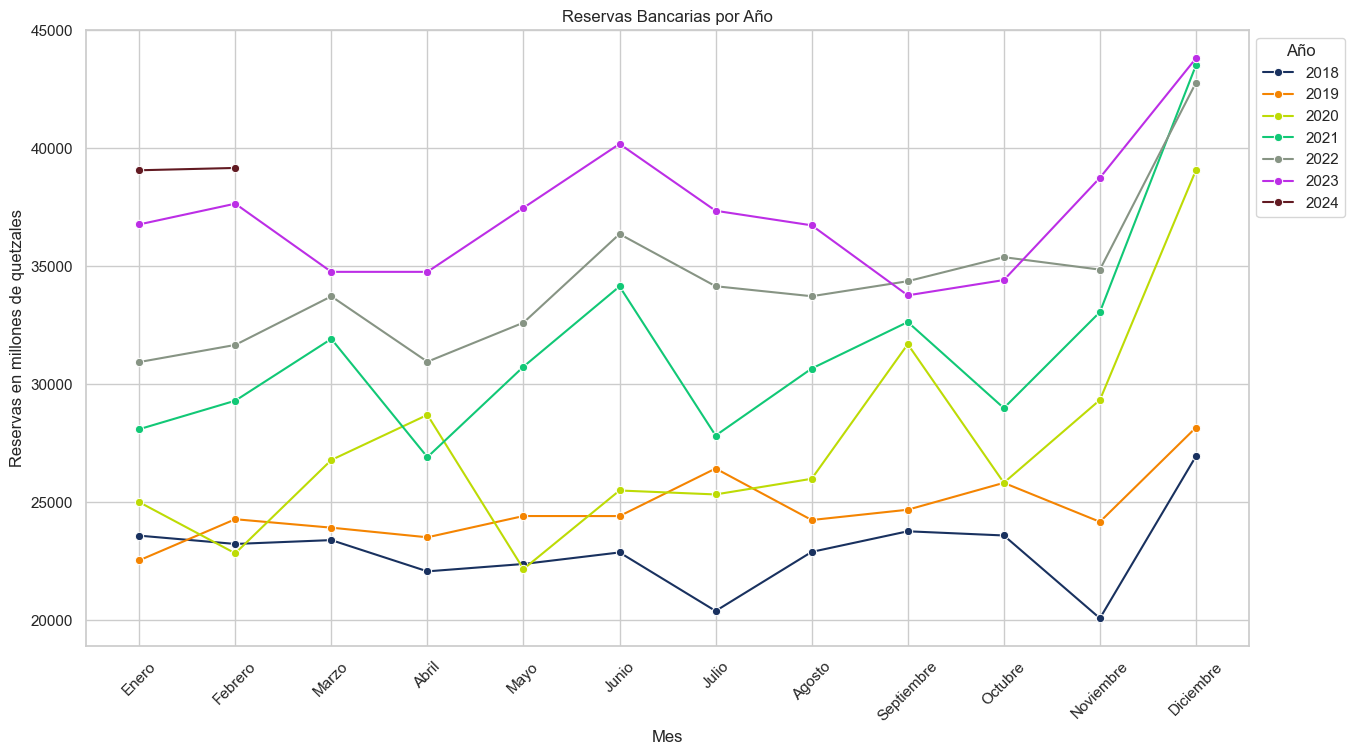
\includegraphics[scale=0.5]{imagenes/reservas_en_guatemala.png}
    \caption{Evolución de la constitución de reservas bancarias en Guatemala.}
    \small{Fuente: Elaboración propia a partir de  datos del Banco de Guatemala.}
    \label{evolucion de reservas}
\end{figure}

%agregar variaciones intermensiales, interanuales y analizar algo de la tendencia


A simple vista, lo primero que podríamos decir es que, en promedio, las reservas bancarias tienden a incrementarse con el tiempo. Por otro lado, es importante resaltar que no hay ningún año en el que las reservas de cualquier mes caigan por debajo del mínimo registrado en los años anteriores. Aun así, sí es posible identificar que, en determinados meses, las reservas son inferiores a las reservas máximas alcanzadas en algún punto de años previos. Esto nos lleva a concluir que aunque las reservas muestran un incremento al concluir cada año, hay momentos específicos dentro del año en los que las reservas bancarias no alcanzan algunos valores observados en periodos previos. Por ejemplo, podemos observar que los valores mínimos de las reservas en 2019, 2020 y 2021 son menores que los máximos registrados en todos los años analizados antes. Los años 2022 y 2023 presentan esta tendencia de manera parcialmente, por lo que, aunque la tendencia no se ha eliminado por completo, parece observarse cierta mejora. \\



Por otro lado, hay que considerar que una perspectiva importante a contemplar es la relación entre las reservas bancarias y la inflación. Se sabe que el aumentar el porcentaje de reservas requeridas puede conllevar a una disminución de los recursos líquidos que las instituciones financieras poseen para la concesión de créditos, induciendo una contracción en la masa monetaria circulante dentro de la economía. Por otro lado, al disminuir el porcentaje,los bancos pueden prestar más, lo que potencialmente provoca una alza en la inflación. Con el fin de analizar las reservas bancarias y la inflación en Guatemala, a continuación un análisis de las variaciones intermensuales absolutas y la evolución de la constitución de reservas en relación con la inflación mensual. 


\subsubsection{Variaciones Intermensuales e Interanuales Absolutas}
En este apartado haremos un análisis descriptivo breve y general de la constitución de reservas en Guatemala en los últimos años y los meses transcurridos del 2024. Comenzaremos por examinar las variaciones interanuales absolutas para luego abordar las variaciones intermensuales absolutas. Posteriormente, buscaremos comparar la constitución de reservas con la dinámica inflacionaria del país, con el objetivo de evaluar cómo ha evolucionado el valor real de las reservas bancarias a lo largo del tiempo y qué efecto ha tenido la inflación sobre las reservas.
\newpage
\begin{figure}[ht!]
    \begin{minipage}{0.5\textwidth}
        \centering
        \begin{center}
Variaciones Interanuales Absolutas en la \\ 
Reserva Bancaria Nacional  en Diciembre \\
de cada año en millones de quetzales\\
\begin{tabular}{
  @{}
  l % Columna de año como texto (o entero sin formato especial de siunitx)
  S[table-format=4.0] % Esto no debería aplicarse a la columna de años; ajuste hecho en la siguiente línea
  S[table-format=-5.1] % Columna de variación con formato numérico
  @{}
}
\toprule
\textbf{{Año}} & \textbf{{Variación}} \\
\midrule
2019 & 1215.3 \\
2020 & 10913.3 \\
2021 & 4448.1 \\
2022 & -740.2 \\
2023 & 1031.4 \\
\bottomrule
\end{tabular}
\end{center}
    \end{minipage}%
    \begin{minipage}{0.5\textwidth}
        Una observación clara y directa es que, entre los últimos seis años, el 2022 destaca por ser el único en registrar una disminución absoluta en la formación de reservas bancarias. Adicionalmente, es notable que la variación en 2020 superó la suma total de las variaciones de los demás años combinados.
    \end{minipage}
\end{figure}
La siguiente tabla muestra las variaciones intermensuales absolutas en la Reserva Nacional Bancaria de Guatemala
\begin{table}[H]
\begin{center}
Variaciones Intermensuales Absolutas en la Reserva Bancaria Nacional \\
de Guatemala en millones de quetzales \footnote{Diferencias intermensuales absolutas en las reservas bancarias en Guatemala.}
\\
\begin{tabular}{
  @{}
  l
  S[table-format=-4.1]
  S[table-format=-4.1]
  S[table-format=-4.1]
  S[table-format=-4.1]
  S[table-format=-4.1]
  S[table-format=-4.1]
  @{}
}
\toprule
\textbf{Mes} & {\textbf{2018}} & {\textbf{2019}} & {\textbf{2020}} & {\textbf{2021}} & {\textbf{2022}} & {\textbf{2023}} \\
\midrule
Ene & 0.0 & -4417.0 & -3162.5 & -10985.4 & -12586.4 & -6011.4 \\
Feb & -352.5 & 1744.7 & -2170.9 & 1208.7 & 725.8 & 879.0 \\
Mar & 163.4 & -357.9 & 3956.4 & 2620.0 & 2060.4 & -2889.7 \\
Abr & -1325.1 & -408.5 & 1913.1 & -5012.1 & -2772.1 & 0.0 \\
May & 312.4 & 901.6 & -6535.6 & 3834.6 & 1655.9 & 2714.6 \\
Jun & 489.8 & -1.8 & 3329.5 & 3402.1 & 3757.9 & 2708.7 \\
Jul & -2481.9 & 2016.6 & -166.8 & -6321.5 & -2213.5 & -2833.8 \\
Ago & 2504.4 & -2184.2 & 664.1 & 2841.0 & -423.7 & -617.8 \\
Sep & 873.8 & 436.8 & 5704.6 & 1971.0 & 636.6 & -2967.4 \\
Oct & -176.9 & 1139.6 & -5874.4 & -3648.9 & 1019.2 & 648.4 \\
Nov & -3510.9 & -1652.2 & 3511.7 & 4071.5 & -527.8 & 4334.7 \\
Dic & 6871.8 & 3997.6 & 9744.1 & 10467.1 & 7927.5 & 5066.1 \\
\bottomrule
\end{tabular}
\end{center}
\caption{Variaciones Intermensuales Absolutas en la Reserva Bancaria Nacional}
\end{table} 
Podemos observar que el 2021 fue el año con el mayor número de variaciones intermensuales positivas. Asimismo, se observa una reducción significativa de las reservas en enero de cada año. Aunque el país incrementa sus reservas en diciembre, la disminución experimentada en enero excede al incremento de diciembre en el 40\% de los casos analizados.\footnote{Esto corresponde a los años 2021 y 2022.} \\


Finalmente, siguiendo en la línea del análisis general de la constitución de reservas en el país, retomamos el gráfico \ref{evolucion de reservas}, pero le incorporamos un nuevo elemento: partiendo de las reservas al inicio de cada año y tomando en cuenta la inflación mensual del país, proyectamos cómo se habrían mantenido constantes, en términos de valor, las reservas a lo largo del año. Esto permite evaluar el valor de las reservas iniciales, y ver si su valor permanece, al menos inalterado, ante la inflación.  Para cada año, elaboramos un gráfico que ilustra dos curvas: la trayectoria real de las reservas bancarias y la proyección ajustada por la inflación de las reservas para reflejar un valor constante. Al ajustar por inflación, podemos evaluar de manera efectiva el poder adquisitivo de las reservas bancarias y cómo este se ha mantenido o variado.

%Posteriormente, en otro análisis que presentamos, retomando los datos de las reservas bancarias mensuales, procedemos a analizar la evolución de estas  ajustadas por inflación. Para cada año bajo, trazamos una curva que refleja la evolución de las reservas después de descontar el impacto de la inflación mensual. Este enfoque nos permite observar la trayectoria de las reservas de una forma más precisa sobre el verdadero valor de las reservas a lo largo del tiempo. 
El  escenario  se enfoca en mantener constante el valor real de las reservas a través del tiempo, compensando la inflación, por lo que se se fija el monto de reservas de enero de cada año y se hace una proyección del monto en quetzales que tiene el mismo valor en cada uno de los próximos meses. En el gráfico \ref{proyeccion reservas inicio de año}, podemos notar que, en términos de valor, cada año se observó un incremento en las reservas comparado con el mes de enero. El año 2018 se caracterizó por tener, excepto diciembre, un valor de reserva inferior al observado en enero. Por el contrario, en 2019, el valor de la reserva superó al de enero durante todos los meses. Los años subsiguientes mostraron una variabilidad en la que, en algunos meses, el valor de las reservas superó al de inicio de año, mientras que en otros meses, disminuyó. Los años 2020 y 2021 se distinguieron por tener una tasa de inflación más baja en comparación con otros períodos; en 2021 fue positiva en todos los meses, a diferencia de otros años donde se registró deflación en algunos meses.

\begin{figure}[H]
  \centering
  \captionsetup{justification=centering}

  % Fila 1
  \begin{subfigure}[b]{0.495\textwidth}
    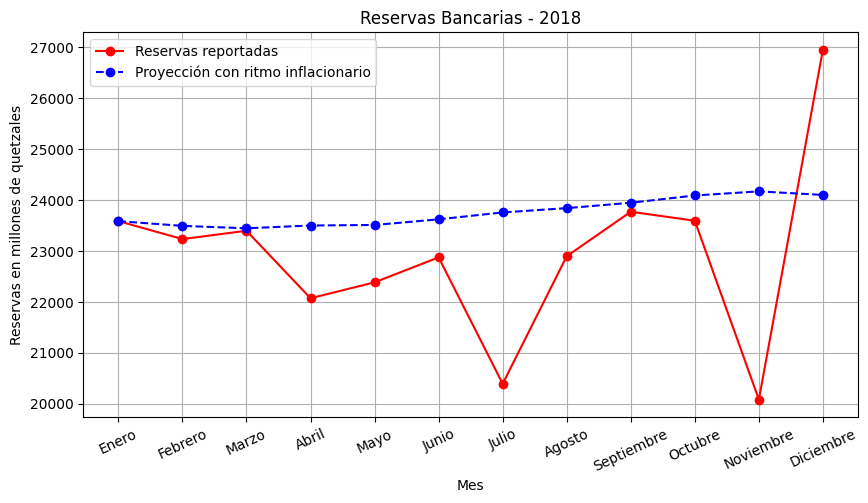
\includegraphics[width=\linewidth]{imagenes/reservas_2018.png}
    \caption{2018}
    \label{proyeccion reservas inicio de año}
  \end{subfigure}
  % No hay espacio intencionalmente entre las figuras para maximizar el tamaño de la imagen
  \begin{subfigure}[b]{0.495\textwidth}
    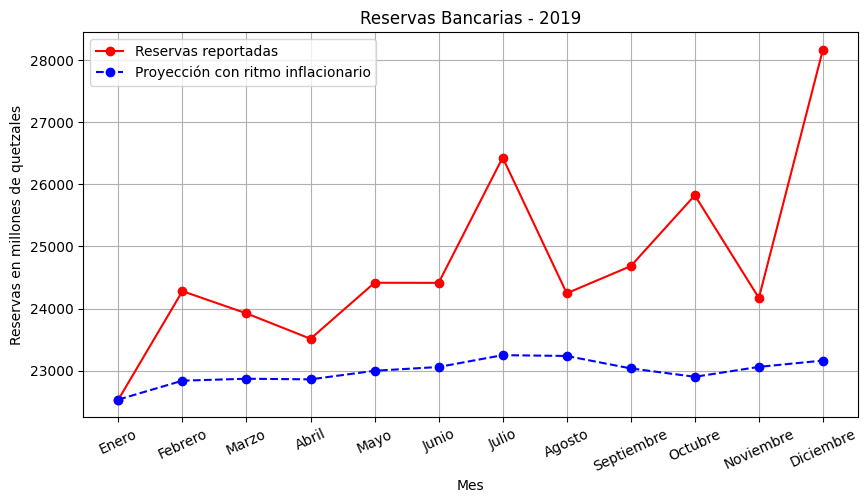
\includegraphics[width=\linewidth]{imagenes/reservas_2019.png}
    \caption{2019}
  \end{subfigure}
  
  % Fila 2
  \begin{subfigure}[b]{0.495\textwidth}
    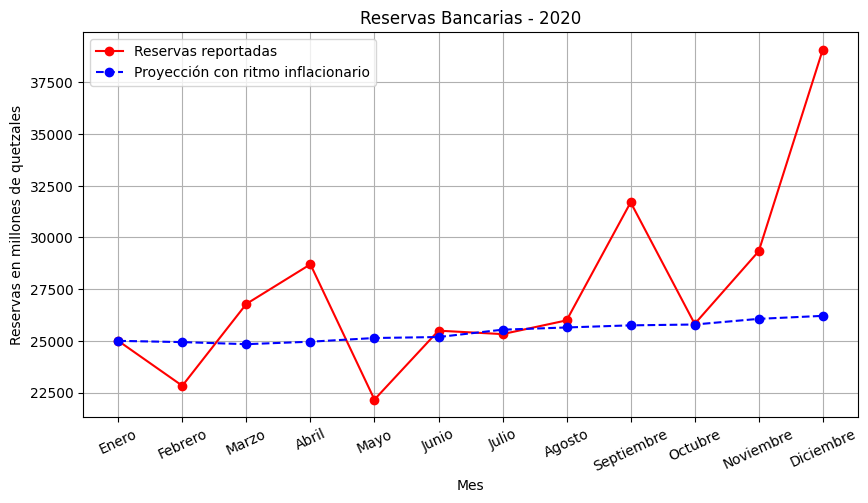
\includegraphics[width=\linewidth]{imagenes/reservas_2020.png}
    \caption{2020}
  \end{subfigure}
  % No hay espacio intencionalmente entre las figuras para maximizar el tamaño de la imagen
  \begin{subfigure}[b]{0.495\textwidth}
    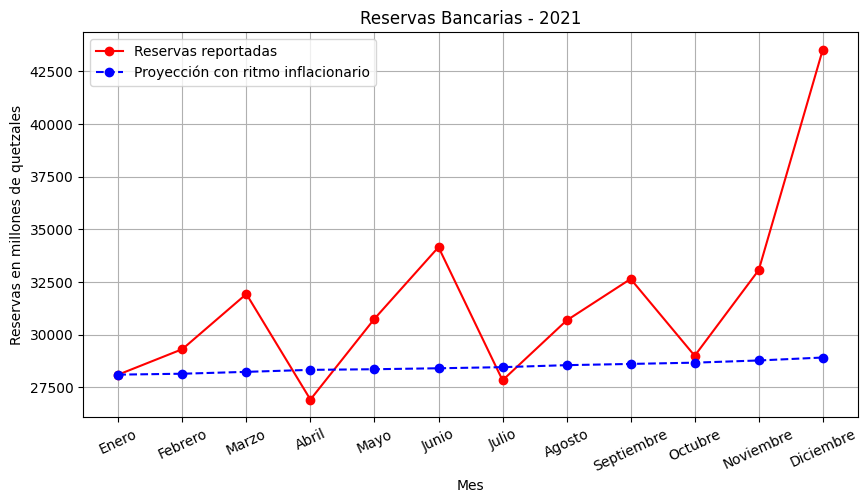
\includegraphics[width=\linewidth]{imagenes/reservas_2021.png}
    \caption{2021}
  \end{subfigure}
  
  % Fila 3
  \begin{subfigure}[b]{0.495\textwidth}
    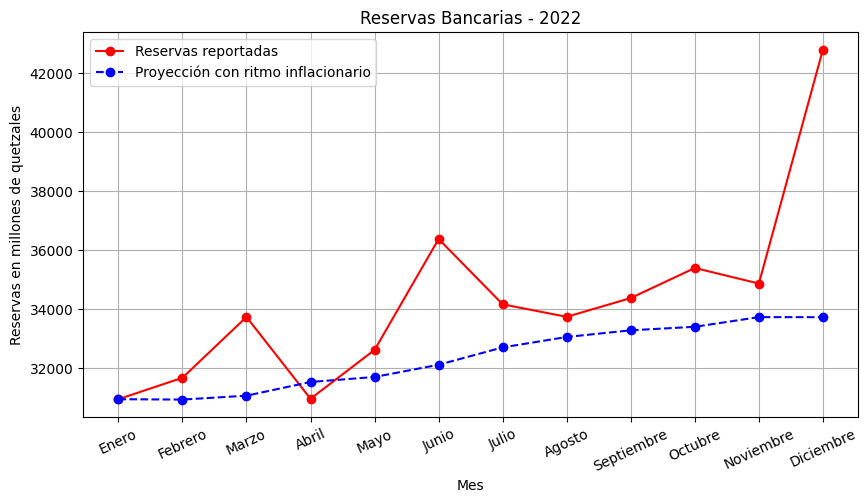
\includegraphics[width=\linewidth]{imagenes/reservas_2022.png}
    \caption{2022}
  \end{subfigure}
  % No hay espacio intencionalmente entre las figuras para maximizar el tamaño de la imagen
  \begin{subfigure}[b]{0.495\textwidth}
    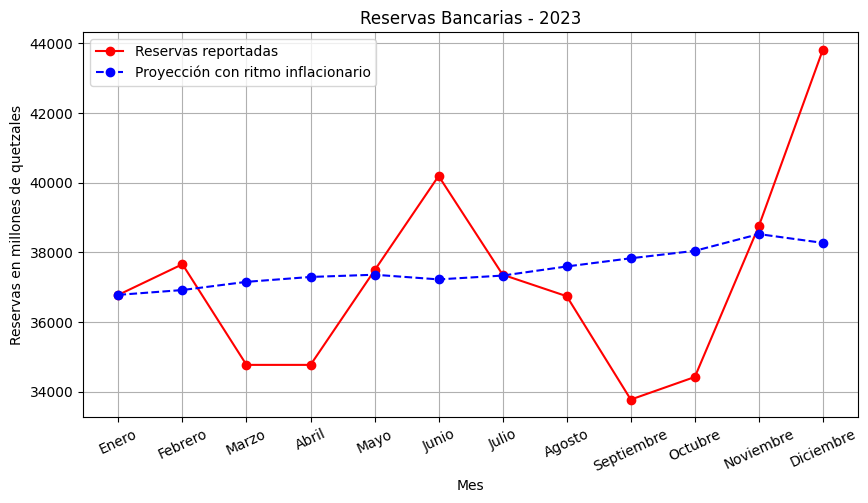
\includegraphics[width=\linewidth]{imagenes/reservas_2023.png}
    \caption{2023}
  \end{subfigure}
\caption{Proyección de valor constante de las Reservas a inicio de año bajo efecto de la inflación}
\end{figure}
\newpage
Observamos que las reservas proyectadas, que se ajustan por inflación de manera progresiva mes a mes, generalmente están por debajo de las reservas reales reportadas. Esto indica que las reservas bancarias no solo han crecido lo suficiente para contrarrestar la inflación, sino que han aumentado en términos de poder adquisitivo.


%En el segundo análisis, en vez de fijar el valor en quetzales de las reservas de enero de cada año, fijamos el valor del dinero en enero de cada año y hacemos una proyección del equivalente en quetzales a las reservas constituidas cada mes según la métrica de valor del dinero de inicio de ese año. Tomando el gráfico \ref{evolucion de reservas}, trazamos la nueva curva para la comparación. Obtenemos las gráficas  \ref{proyeccion retro}.

%Al ajustar las reservas reportadas mes a mes, eliminando el efecto de la inflación, buscamos evaluar cómo se hubieran comportado las reservas si se hubiera reservado lo mismo en valor, y no hubiese existido el efecto de la inflación. Podemos observar, como era de esperarse, que el efecto de la inflación\footnote{Datos de inflación recuperados del Instituto Nacional de Estadística} provocó una desaceleración, en muchos casos, del valor adquisitivo de las reservas. Los años 

%Podemos observar que en ciertos puntos  el poder adquisitivo real de las reservas parece disminuir con el tiempo (esto es claro en los puntos en los que la curva \textcolor{red}{roja} está por debajo de la curva \textcolor{blue}{azul}. Los años 2019, 2021 y 2022 destacan por estar, en la mayoría de meses del año, en temas de consitución de reservas, por encima de las reservas en quetzales requeridas para igualar al valor de las reservas de inicio de año. Es decir, durante la mayoría de los meses de esos años, el valor de las reservas aumentó respecto de inicio de año. Por otro lado, en 2018 podemos observar que solamente en septiembre, octubre y diciembre, las reservas crecieron en valor respecto de enero. Los años 2020 y 2023 tienen un comportamiento más fluctuante en cuanto al crecimiento en valor. En general, el lector podrá notar que estas proyecciones se asemejan mucho a las realizadas en el primer análisis. Esto ocurre pues la perspectiva de ambos análisis fue evaluar la constitución de reservas bajo la óptica de la situación a inicio de cada año, siendo en el primer análisis, una comparativa entre el dinero guardado y el dinero necesario a guardar para mantener el valor de enero, mientras que en el segundo, una evaluación del impacto de la inflación en cada mes.

%\begin{figure}[H]
  \centering
  \captionsetup{justification=centering}

  % Fila 1
  \begin{subfigure}[b]{0.495\textwidth}
    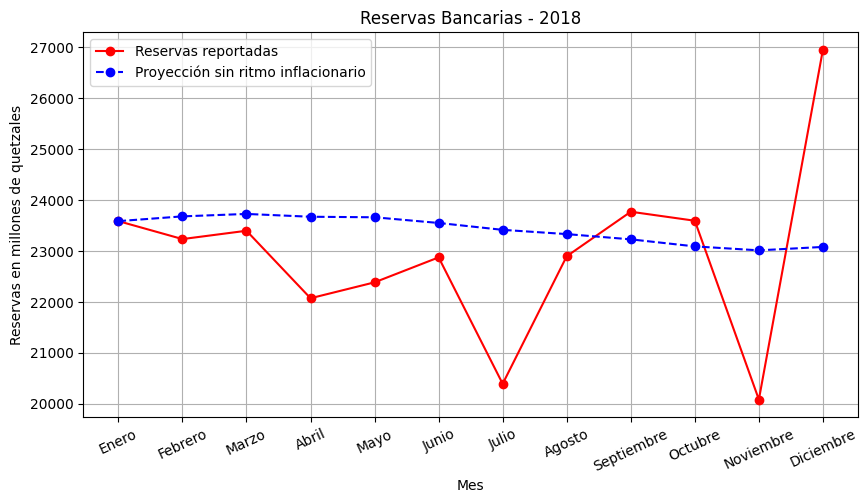
\includegraphics[width=\linewidth]{imagenes/retro_2018.png}
    \caption{2018}
    \label{proyeccion retro}
  \end{subfigure}
  % No hay espacio intencionalmente entre las figuras para maximizar el tamaño de la imagen
  \begin{subfigure}[b]{0.495\textwidth}
    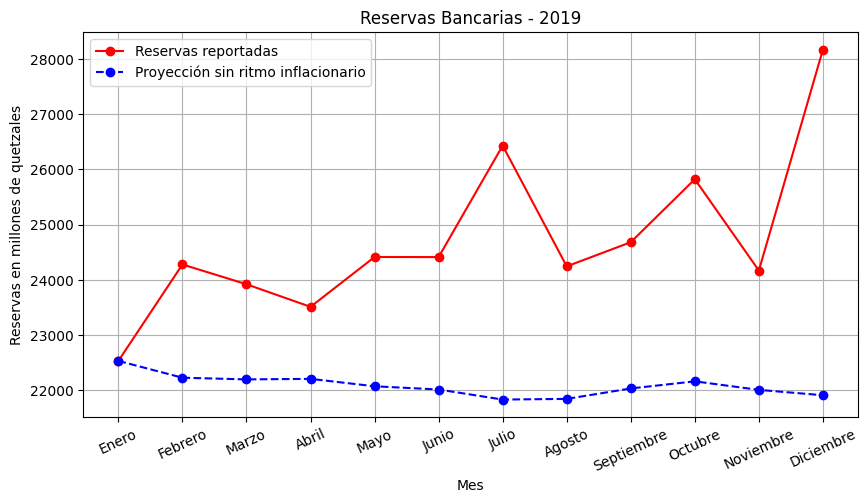
\includegraphics[width=\linewidth]{imagenes/retro_2019.png}
    \caption{2019}
  \end{subfigure}
  
  % Fila 2
  \begin{subfigure}[b]{0.495\textwidth}
    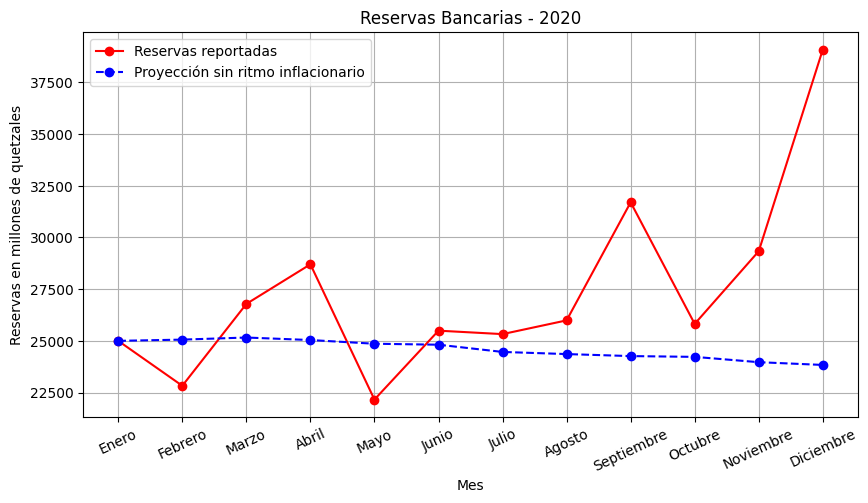
\includegraphics[width=\linewidth]{imagenes/retro_2020.png}
    \caption{2020}
  \end{subfigure}
  % No hay espacio intencionalmente entre las figuras para maximizar el tamaño de la imagen
  \begin{subfigure}[b]{0.495\textwidth}
    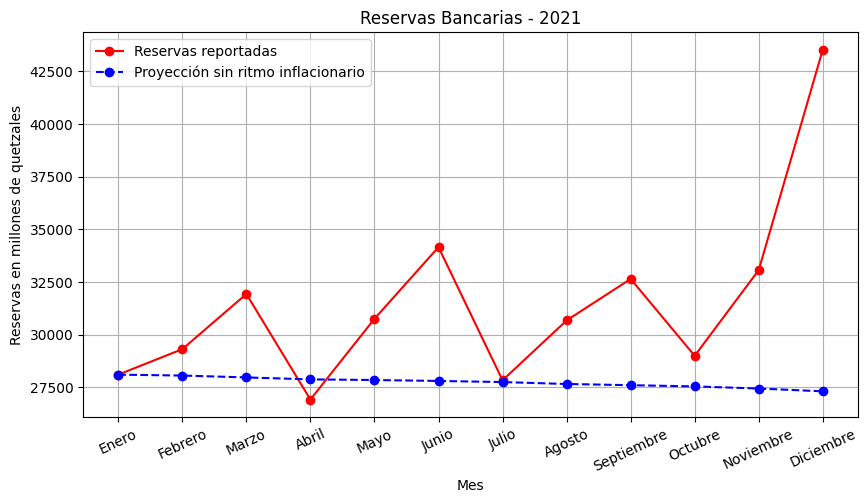
\includegraphics[width=\linewidth]{imagenes/retro_2021.png}
    \caption{2021}
  \end{subfigure}
  
  % Fila 3
  \begin{subfigure}[b]{0.495\textwidth}
    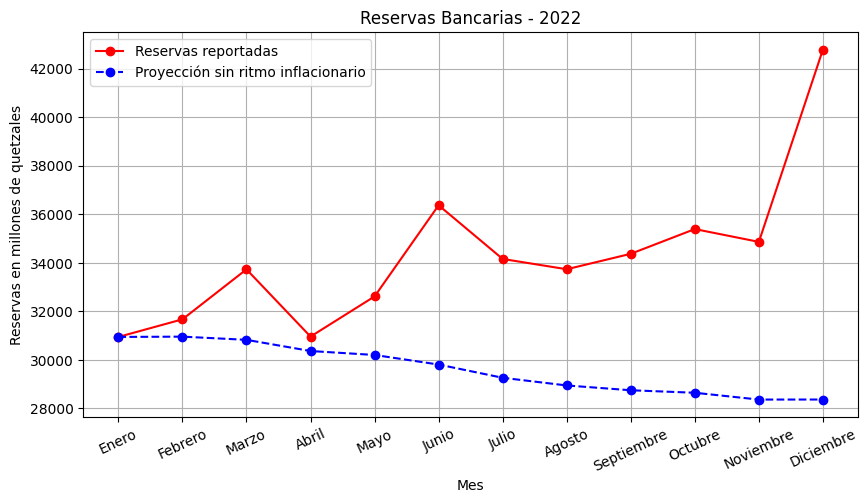
\includegraphics[width=\linewidth]{imagenes/retro_2022.png}
    \caption{2022}
  \end{subfigure}
  % No hay espacio intencionalmente entre las figuras para maximizar el tamaño de la imagen
  \begin{subfigure}[b]{0.495\textwidth}
    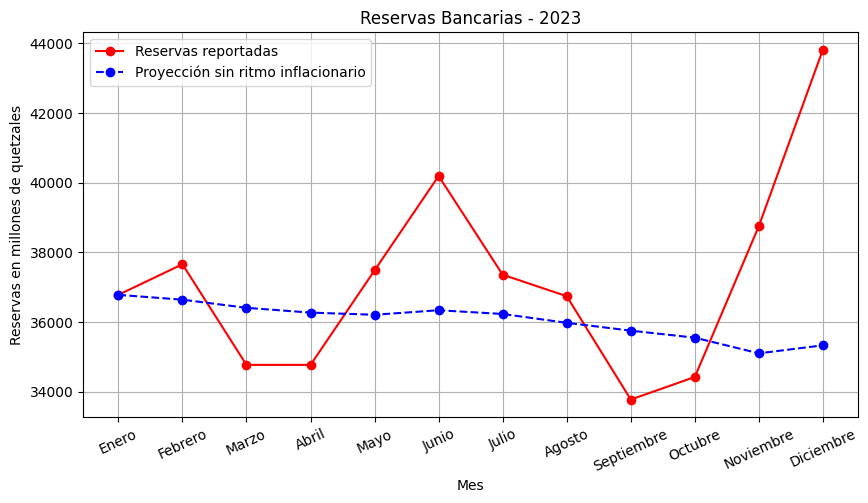
\includegraphics[width=\linewidth]{imagenes/retro_2023.png}
    \caption{2023}
  \end{subfigure}
\end{figure}


\subsection{Política Monetaria y Crediticia en Guatemala}
Guatemala ha implementado políticas monetarias y crediticias orientadas a fortalecer el sistema financiero y bancario  buscando adaptarse a estándares internacionales. Pondremos principal atención a la Resolución JM-47-2022, la cual se enfoca en actualizar el marco regulatorio para la valoración de activos. En la normativa, se establece un régimen de clasificación de activos y de reservas basado en la capacidad de pago y cumplimiento del deudor. Esta normativa busca gestionar el cumplimiento de reservas y la correcta gestión de riesgo de créditos. Esta normativa fue emitida por la Junta Monetaria de Guatemala el 25 de mayo de 2022, para entrar en vigencia a partir del 01 de enero de 2023. Claramente, esta política permite administrar mejor el riesgo en los bancos y respaldar el sistema financiero mediante la constitución de reservas bancarias. Sin embargo, como veremos más adelante, esto le exige a los bancos reservar cierto dinero que hasta antes de la política, no se reservaba, provocando así que las entidades bancarias se vean en la posición de ya sea aumentar tasas a los créditos o bien, mantener precios pero correr el riesgo de perder rentabilidad.

\subsubsection{JM-47-2022}
La Resolución JM-47-2022 introduce un marco regulatorio avanzado para la gestión del riesgo de crédito focalizándose en una metodología prospectiva para la evaluación de la capacidad de pago de los deudores y la adecuada clasificación de activos en función del riesgo. Técnicamente, esta normativa impone a los bancos el cálculo de provisiones basadas en la estimación de pérdidas esperadas, integrando conceptos como la Probabilidad de Incumplimiento (PI), la Pérdida Dado el Incumplimiento (PDI) y la Exposición al Momento del Incumplimiento (EMI), para refinar la estimación de reservas específicas y dinámicas. Específicamente, exige una valoración precisa de activos crediticios, incluyendo la alineación de activos crediticios bajo un enfoque de refinanciación y reestructuración, y la categorización de riesgos en activos según un modelo que contempla variables macroeconómicas y del mercado. A nivel operativo, los bancos deben, dependiendo del tipo de crédito y de la categoría del créditohabiente, reservar un porcentaje del monto del crédito que está otorgando. El lector puede consultar el Anexo \ref{categorias} para más información del cálculo de categorías. Puntualmente, los bancos deben calcular sus pérdidas esperadas, por el riesgo de crédito, con la fórmula
\begin{align}\label{formula pe}
    PE &= (PI) \times (PDI) \times (EMI).
\end{align}
Las probabilidades de incumplimiento son dadas en la Resolución de la normativa y se dividen entre probabilidades para créditos empresariales y créditos de productos, habiendo, posteriormente a esta división, una segmentación por tipo de crédito. El lector puede consultar el Anexo \ref{categorias} si desea ver algunas tablas de probabilidad de incumplimiento según tipo de crédito. Así mismo, la pérdida dado el incumplimiento se presenta según tipo de garantía del crédito y categoría del créditohabiente en el documento de la resolución. Se puede consultar la Resolución de la Normativa para más información.\footnote{El enlace a la resolución se encuentra en la bibliografía de este documento.} Finalmente, la exposición al momento de incumplimiento corresponde al saldo pendiente del crédito al momento del cálculo de las reservas. 

De esta forma, los bancos, con cada período de pago del crédito, deberán reservar un porcentaje de este de acuerdo a la probabilidad de incumplimiento y la pérdida dado el incumplimiento. Nótese que estos dos parámetros dependen del tipo y garantía del crédito y la categoría del créditohabiente. Además, la reserva, en quetzales, está dada por la fórmula \ref{formula pe}. 

\subsection{Desafíos actuales en la gestión del riesgo de crédito}
% aca hacer algun estudio de series de timepo para ver la estabilidad que se maneja actualmente y la esperada
% tambien se podria analizar la perspectiva de la jm47 en cuanto a garantizar reseras pero tambien cuidar a nivel micro a los creditohhabientes medinate un estudio de sus condiciones economicas

%vincular esto con el analisis de reservas e inflacion que se hizo antes

Con el nuevo paradigma de establecimiento de precios de crédito inducido por la JM47-2022, nos encontramos ante una situación que puede ser vista desde diferentes aristas.  Para analizar los desafíos actuales en la gestión del riesgo de crédito, iniciaremos revisando los datos de inflación y la formación de reservas, referenciados en los gráficos \ref{proyeccion reservas inicio de año} y \ref{proyeccion retro}. Aplicaremos un Modelo autorregresivo integrado de media móvil (ARIMA) para proyectar las reservas, conservando en el análisis tanto la curva de reservas iniciales del año como una proyección ajustada, excluyendo el efecto inflacionario. Esto nos permitirá evaluar cómo la acumulación de reservas se compara con las tendencias inflacionarias, brindando así una perspectiva cuantitativa sobre el asunto. Además, en el ámbito de las reservas bancarias, enfrentamos el reto de equilibrar la rentabilidad bancaria con la salud financiera de los créditohabientes. Por ende, el establecimiento de precios para el crédito no solo responde a criterios de rentabilidad y ganancia económica; representa también una cuestión de gran relevancia social y humana.

\subsubsection{Modelo autorregresivo integrado de media móvil: Análisis del desafío actual de Inflación y Reservas Bancarias}
Utilizando Python, ver anexo \ref{codigo sarima}, haremos una proyección de las reservas. Este estudio busca evaluar cuál sería el escenario futuro si se siguiera con la constitución de reservas bajo las normativas previas a la JM47-2022. La proyección se hará utilizando un Modelo SARIMA. Los parámetros no estacionarios utilizados para el modelo fueron $(p,d,q) = (1,1,1)$ y los  estacionarios, $(P,D, Q, S) = (0,0,2,12)$. Los parámetros fueron encontrados utilizando la librería estadística \textit{pmdarima} de Python. Los resultados de las proyecciones se muestran a continuación. 
\begin{figure}[H]
    \centering
    \begin{minipage}{.85\textwidth}
        \centering
        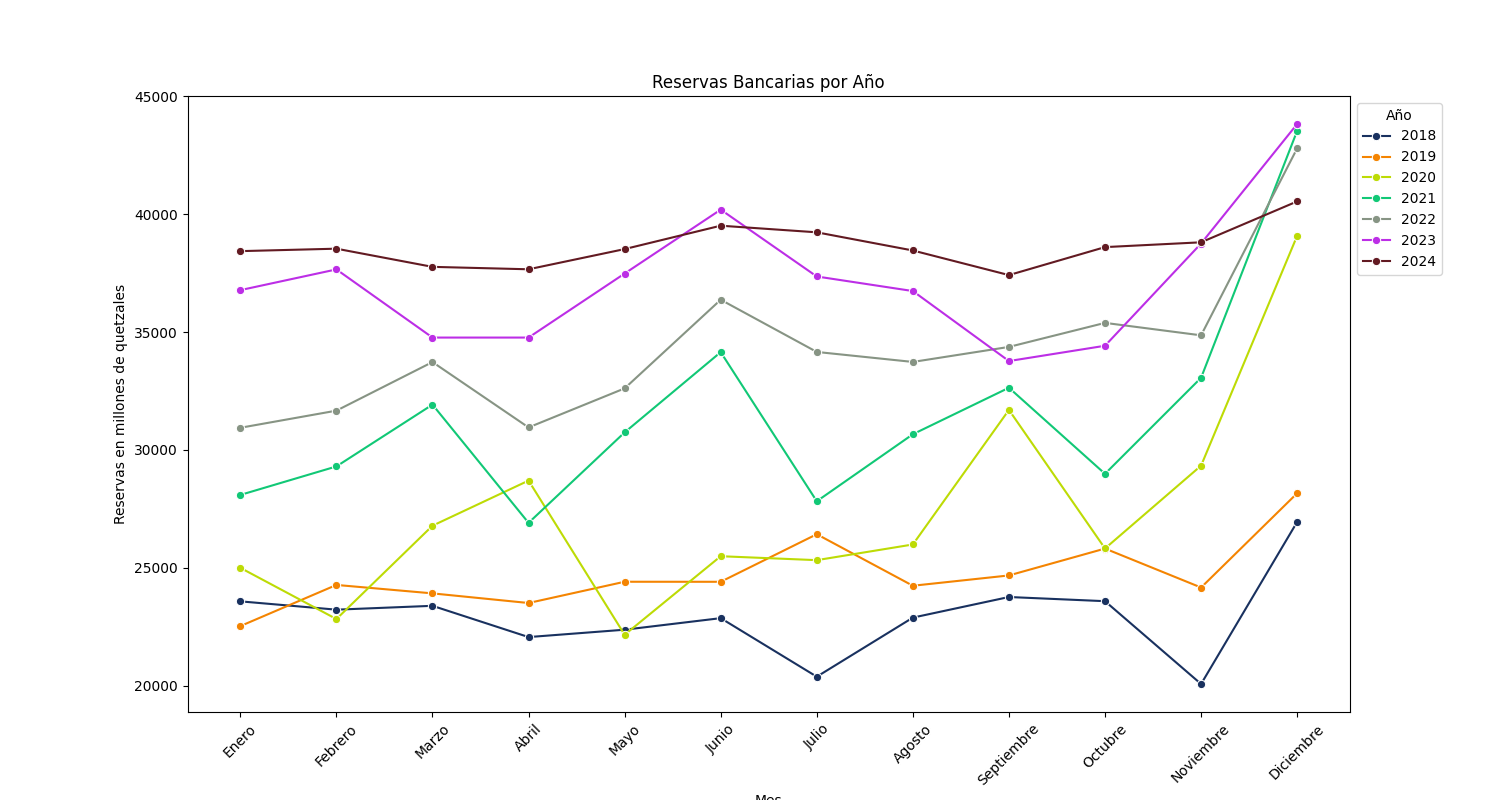
\includegraphics[width=\linewidth]{imagenes/prediccion_reservas_sarima.png}
        \caption{Predicción de las Reservas Bancarias 2024 usando modelo SARIMA}
        \label{fig:sarima-prediction}
    \end{minipage}%
    \begin{minipage}{.15\textwidth}
        \centering
        {\scriptsize 
        \begin{tabular}{lc}
            \hline
             & Valor (en quetzales) \\
            \hline
            MSE & 3,671,571.71 \\
            RMSE & 1,916.13 \\
            MAE & 1,558.97 \\
            AIC & 1,136.75 \\
            % BIC & 1,147.14 \\
            \hline
        \end{tabular}
        }
        %\captionof{table}{\scriptsize Nivel de error del modelo.}
        \label{proyeccion sarima}
    \end{minipage}
\end{figure}
En el gráfico referido como \ref{proyeccion sarima}, se observa que la proyección para las Reservas Bancarias al cierre de 2024 es inferior a las registradas en los años 2021, 2022 y 2023. A lo largo de 2024, sin embargo, las proyecciones sugieren que las Reservas podrían exceder los niveles de años anteriores. Cabe destacar que la tasa de acumulación de Reservas en diciembre de 2024 es menor comparada con la de diciembre de años previos, y la tendencia general de aumento y disminución de Reservas en 2024 muestra una curva más aplanada.

El propósito de este gráfico no es meramente comparativo o prescriptivo, sino que busca analizar la posible situación de las Reservas Bancarias bajo la continuación de las normativas actuales. Este análisis pretende resaltar la relevancia de mantener o ajustar la normativa vigente para reflejar las necesidades económicas. Aunque las metas de Reservas están influenciadas por diversos factores y objetivos económicos nacionales, un análisis más completo podría beneficiarse de incorporar factores adicionales, como la inflación. En términos generales, se puede concluir que, bajo el ritmo actual, las Reservas podrían resultar insuficientes al final del año, indicando la necesidad de modificar las directrices para su constitución. Además, para acelerar la formación de Reservas, alineándolo con los objetivos económicos del país, sería esencial mitigar el riesgo de crédito, posiblemente mediante el incremento de los requisitos para las reservas.
 %reservas bancarias

\section{Fundamentos e Innovación para la Gestión del Riesgo de Crédito}

% algo sobre las leyes en cuanto a precios de creditos
\subsection{Modelo matemático avanzado: gestión de riesgo de crédito y optimización de reservas bancarias}

Considerando la Resolución JM-47-2022, el propósito de este modelo matemático avanzado es definir analíticamente un intervalo donde cada punto representa un posible precio de crédito. Dicho intervalo será construido hallando, en primera instancia, una tasa mínima para dejar el margen financiero de un crédito a cero, pero cumplir con los costos pasivos y la constitución de reservas, y como extremo superior del intervalo, una tasa máxima para el precio de crédito, la cual será encontrada resolviendo el problema de optimizar el margen financiero sujeto a dos condiciones: la certeza de la constitución de reservas y el decremento o mantenimiento del nivel de saturación del créditohabiente. A continuación, demostraremos que, aplicando una función convexa sobre este intervalo,los bancos pueden encontrar el punto óptimo de precio en dicho intervalo. Esta estrategia proporciona a las instituciones una metodología para cumplir con los requisitos de constitución de reservas, a la vez que protege la salud financiera de los créditohabientes y asegura su propia rentabilidad. Al elegir adecuadamente su función convexa de personalización de precios, los bancos pueden alcanzar sus objetivos específicos, ofreciendo así una solución integral que garantiza las necesidades de todas las partes involucradas.

\subsubsection{Formulación matemática}
Comenzaremos por definir la notación que se utilizará. Supondremos que se tiene un créditohabiente con crédito al cual se le identifican características en distintos periodos de tiempo. La notación a utilizar es la siguiente.
\begin{align*}
    C_n & \text{: capital adeudado en el tiempo $n$} & MF_n & \text{: margen financiero en el tiempo $n$} \\
    t_n & \text{: tasa otorgada en el tiempo $n$} & D & \text{: desembolso neto} \\
    \alpha & \text{: } \frac{\text{tasa pasiva} + \text{FOPA}}{1- \text{encaje}} & PI(x) & \text{: función probabilidad de incumplimiento} \\
    c_1^n & \text{: categoría interna del créditohabiente en el tiempo $n$} & PDI(x) & \text{: función pérdida dado incumplimiento} \\
    c_2^n & \text{: categoría externa del créditohabiente en el tiempo $n$} & PE_n & \text{: Pérdida esperada en el tiempo $n$} \\
    p & \text{ plazos para el crédito} & I_n & \text{: ingresos mensuales en el tiempo $n$} 
\end{align*}

\subsubsection{Modelación del margen financiero}

Una medida que las instituciones bancarias deben cuidar es su viabilidad financiera. Procedemos a modelar el margen financiero primer punto para la construcción del modelo en el cual estamos interesados.  El margen financiero en el $n$-ésimo punto del tiempo, al cual llamaremos $MF(n)$ está dado por
\begin{align*}
    MF(n) &= C_n(t_n-\alpha) - R(n)
\end{align*}
donde $R(x)$ es la función que a cada créditohabiente le asigna el monto que provoca en reservas en función de su categoría interna, externa, pérdida dada el incumplimiento y su exposición al momento de incumplimiento en el tiempo $x$. 

La atención ahora se centra en definir la función de reservas $R$. Para esto, tenemos
\begin{align*}
    R(x, n) &= PI(x)\cdot PDI(x) \cdot C_n
\end{align*}


De acuerdo a las indicaciones dadas en la JM-47-2022, y como se muestra en el anexo \ref{categorias} y en la \href{https://banguat.gob.gt/sites/default/files/banguat/Publica/Res_JM/2022/Res_JM-47-2022.pdf}{Resolución de la JM47-2022}, página 11, según la categoría del créditohabiente, la función de reservas estará bien definida. Por tanto, la función de reservas es el producto de dos funciones por partes definidas en la Resolución de la JM47-2022.\\

Por el momento, hemos modelado una función relacionada al estudio de la rentabiliad de una institución bancarias, pero aún no hemos modelado nada que nos permita vincular toda esta información con las condiciones de los créditohabientes. Para ello, modelaremos la Relación Cuota Ingreso (RCI) de un créditohabiente. La razón por la cual se eligió modelar el RCI es porque es una medida que transmite mucha información sobre la situación financiera de una persona. Además, es bien conocida que las instituciones bancarias toman esta medida como un parámetro o argumento en sus scores para otorgamiento de créditos. Podemos modelar el $RCI$ de un créditohabiente como
\begin{align*}
    RCI &= \frac{d_n}{I_n}.
\end{align*}

Para este punto, que ya tenemos modelado el margen financiero de una institución bancaria y al Relación Cuota Ingreso de un créditohabiente. El siguiente paso será construir una clústerización de los créditohabientes de acuerdo a su nivel de saturación medido en el RCI. Un ejemplo de posible clusterización es la siguiente
\begin{table}[H]
    \centering
    \begin{tabular}{|c|l|}
        \hline
        \textbf{Nivel de RCI (x)} & \textbf{Interpretación} \\
        \hline
        $x \leq 0.4$ & Adecuado \\
        $0.5 < x \leq 0.6$ & En ruta de alta saturación \\
        $0.6 < x \leq 0.7$ &  Alta saturación \\
        $x > 0.7$ & Extrema saturación \\
        \hline
    \end{tabular}
    %\caption{Ejemplo de posibles interpretaciones del RCI}
    \label{clusters rci}
\end{table}
\newpage
Se ha mencionado con anterioridad que se busca relacionar las condiciones de un créditohabiente, que en este caso son medidas a través del RCI, y el margen financiero. Claramente, parte del problema es desarrollar y resolver un problema de optimización entre la rentabilidad y el riesgo al momento de otorgar un crédito. De esta forma, para aplicar  ecuación del RCI en el problema de optimización, en lugar de enfocarnos en el RCI total de un créditohabiente, nos centraremos en analizar cómo un crédito nuevo impactaría en el RCI actual. Así, si representamos con $RCI'$ al RCI asociado únicamente con el nuevo crédito, y bajo la suposición de un cálculo de interés compuesto y una amortización fija, llegamos a
\begin{align*}
    RCI' &= \frac{Dt_n(1+t_n)^p}{I_n((1+t_n)^p-1)}.
\end{align*}

Para este punto, tenemos todo lo necesario para plantear un problema matemático de optimización. Procedemos a plantear y resolver el problema de optimización dado por
\begin{center}
    \textit{Maximizar el margen financiero sujeto a la constitución de reservas y decremento o mantenimiento del nivel de saturación de los créditohabientes.}
\end{center}
Una vez encontrado el maximizador, encontraremos el menor precio al que se puede otorgar un crédito para dejar el margen financiero a cero, manteniendo las reservas y los costos pasivos. Con estos dos valores (la tasa maximizadora y la menor tasa), construiremos un intervalo, que corresponderá al intervalo de precios posibles que le corresponde a un créditohabiente. Posteriormente, demostraremos que bajo ciertas condiciones, podemos personalizar el precio de los créditos para cuidar la salud financiera de los créditohabientes y garantizar la rentabilidad de las instituciones bancarias.

\subsection{Optimización: equilibrio riesgo y rentabilidad}
Procedemos a plantear el problema de optimización mencionado anteriormente.

\subsubsection{Problema de optimización}
El problema a resolver, suponiendo el plazo de tiempo es fijo, es
\begin{align*}
    \max MF \text{ sujeto a } \beta \leq RCI \leq \gamma,
\end{align*}
donde $\beta$ y $\gamma$ serán determinadas de acuerdo al clúster de $RCI$  que se determine para el créditohabiente.\footnote{Ver tabla \ref{clusters rci}} Como se había mencionado anteriormente, la condición para la optimización se dará sobre el $RCI'$, la proporción del ingreso del créditohabiente en la cual aumentará el endeudamiento actual de la persona ante un crédito, por lo que podemos replantear el problema como
\begin{align*}
    \max MF \text{ sujeto a } 0 \leq RCI' \leq \gamma - RCI.
\end{align*}

\subsubsection{Solución al problema de equilibrio}
De la condición $MF \geq 0$ llegamos a
\begin{align*}
    t_n &\geq \frac{\Delta R}{C_n-C_{n-1}} + \alpha.
\end{align*}
Sin embargo, si consideramos que queremos personalizar el precio para un crédito nuevo, entonces $C_0 = 0$ y $C_1 = D$, donde $D$ es el desembolso neto del crédito. Además, $\Delta R = R_0$, la reservas correspondientes al cliente según su categoría. De esto, podemos encontrar la menor tasa a la cual se puede otorgar el crédito para dejar el margen financiero a cero, pero garantizar la constitución de reservas y la cobertura de los pasivos. Esto es, 
\begin{align*}
    t &\geq R_0 +\alpha.
\end{align*}
Por otro lado, procedemos a encontrar la tasa máxima a la cual se puede otorgar el crédito maximizando el margen financiero, pero manteniendo el nivel de saturación del cliente. Para resolver el problema de optimización, emplearemos la técnica de optimización convexa.  \\
La función a maximizar es
\begin{align}\label{funcion a optimizar}
    D(t-R(c_1, c_2)-\alpha), \footnote{ donde $c_1$ y $c_2$ son las categorías internas y externas iniciales del créditohabiente. Al decir interna, nos referimos a la categoría del créditohabiente dentro de la institución financiera que está implementando el modelo. La externa se refiere a la categoría en otras instituciones.}
\end{align}
Y la función de restricción es
\begin{align*}
    0 \leq RCI' \leq \gamma - RCI,
\end{align*}
que equivalentemente puede expresarse como
\begin{align}\label{restriccion optimizacion}
    0 \leq \frac{Dt(1+t)^p}{I((1+t)^p-1)} &\leq \gamma - RCI.
\end{align}
Para optimizar bajo las restricciones, supondremos que el plazo $p$ del crédito es dado. Además, nótese que los ingresos $I$, el desembolso neto $D$, las categorías $c_1$ y $c_2$; los pasivos $\alpha$ y el $RCI$ son constantes para un punto fijo en el tiempo (que corresponde al tiempo en el que se solicita el crédito y el modelo es aplicado para encontrar un precio para dicho crédito). Por tanto, tenemos una optimización en una dimensión para la tasa $t$. \\ 
Notemos que la función
\begin{align}\label{mu}
    \mu(t) &= \frac{Dt(1+t)^p}{I((1+t)^p-1)},
\end{align}
siempre que $t\neq 0$ (lo cual siempre ocurrirá en el contexto de nacimiento de créditos), está bien definida. Además, $\mu(t)$ es derivable para todo $t\neq 0$ y 
\begin{align*}
    \frac{d\mu}{dt} &= \frac{D}{I}\left( \frac{(1+t)^{2p} - (1+t)^p-pt(1+t)^{p-1}}{((1+t)^p-1)^2} \right) \geq 0,
\end{align*}
para $p\geq 6$ (para ver la demostración de esta desigualdad, diríjase al anexo \ref{demostracion derivada}). Por tanto, $\mu(t)$ es creciente. Además, el conjunto $S$ dado por
\begin{align*}
    S &= \left\lbrace x \in \mathbb{R} \hspace{0.15cm} | \hspace{0.15cm} \mu(x) \leq \gamma - RCI \right\rbrace
\end{align*}
es convexo. (Para ver la demostración de esta aseveración, diríjase al Anexo \ref{demostracion convexidad}). Por tanto, el conjunto de restricciones para la optimización es convexo. Además, la función \ref{funcion a optimizar}, es decir, la función objetivo, dado que $R(c_1,c_2)$ queda plenamente definida por las reglas establecidas en la JM47-2022 y $\alpha$ es conocido, es una función lineal, que claramente, es convexa. Por tanto, podemos aplicar la técnica de optimización convexa. Esto nos permite concluir que todo máximo local será un máximo global sobre el conjunto de maximizadores viables para el problema. Finalmente, dado que \ref{funcion a optimizar} es creciente\footnote{Nótese que su derivada, una vez $R(c_1,c_2)$ y $\alpha$ son conocidos, es igual a $D$, el desembolso neto, que claramente es positivo.}, y el espacio de optimización convexo, el máximo ocurrirá en la frontera, por tanto, la tasa maximizadora es $t = \gamma - RCI$. Por tanto, dada una persona que solicita un crédito, el intervalo de posibles tasas para el crédito está dado por
\begin{align*}
    \left[ R +\alpha, \mu^{-1}(\gamma - RCI) \right].
\end{align*}

Es decir, hemos encontrado una manera de que a cada solicitante de un crédito, se le construya un intervalo de posibles precios. Este intervalo son todos los precios que tienen sentido para el crédito pues en dicho intervalo, el margen financiero es creciente y la saturación del cliente, medida en RCI, se mantiene o disminuye. De esta manera, lo hace falta es encontrar un punto en el intervalo que corresponderá al precio final del crédito. El precio final dependerá de muchos factores adicionales, los cuales la institución financiera que esté otorgando el crédito deberá determinar. Estos factores pueden ser sus metas de Tasa Promedio Ponderada, su situación financiera actual, promociones de crédito específicas, etc. Por tanto, nos limitaremos a dar condiciones suficientes bajo las cuales, una vez elegidos los factores adicionales por parte de la institución financiera, se puede determinar el precio. 

\subsection{Determinación puntual de Precio de Crédito}
A continuación, mostraremos condiciones suficientes para, una vez construido el intervalo asociado al solicitante de un crédito, se pueda identificar un punto que determinará el precio final del crédito. \\
\begin{mdframed}[linewidth=1pt,linecolor=black] 
\textbf{Teorema: Función de determinación de precio.} \\
Consideremos la solicitud de un crédito dada por un agente al que llamaremos $A$ hacia una institución financiera regida bajo las normativas indicadas por la JM47-2022. Supongamos que la institución financiera desea personalizar sus precios bajo el modelo mostrado en la sección anterior, y sea $[a,b]$ el intervalo de precio asociado al agente $A$. Entonces, cualquier función sobreyectiva sobre $[a,b]$ puede ser adaptada para encontrar el precio del crédito y satisfacer los requerimentos determinados por la institución financiera, siempre que el agente $A$ tenga un nivel de morosidad para el cual el intervalo $[a,b]$ tenga sentido  y los requerimentos sean lógicos.
\end{mdframed} 
\textit{Demostración.} \\
Supongamos que $A$ es un agente solicitante de un crédito y $[a,b]$ es su intervalo\footnote{Al decir que el intervalo tenga sentido, nos referimos a que $a\leq b$. Puede ocurrir que el intervalo no tenga sentido si el nivel de mora es tan alto que sus reservas de crédito induzcan a un precio mayor al que el agente puede pagar según sus condiciones de RCI, en cuyo caso ocurriría $a>b$ y $[a,b]$ no tienen sentido.} de precio asociado construido según el modelo explicado en la sección anterior. Sea $\Omega$ el conjunto de pares ordenados que representan las categorías y el RCI de los créditohabientes y supongamos que hay $m$ requerimentos lógicos determinados por la institución financiera para sus créditos \footnote{Incluyen requerimentos de convergencia a una Tasa Promedio Ponderada específica, el cumplimiento de cierto ingreso financiero establecido como meta para la institución, el cumplimiento de ciertas condiciones para una oferta comercial, etc.}. Todo requerimento lógico puede ser representado mediante alguna de las siguientes: 
\begin{align*}
    \forall (x_i,y_i) &\in S_i, \text{ se cumple } \xi_i \leq f(x_i, y_i) \leq \delta_i, \text{ o bien,}\\
    \forall (x_i,y_i) &\in S_i, \text{ se cumple } \xi_i < f(x_i, y_i) < \delta_i, \text{ o bien,} \\
    \forall (x_i,y_i) &\in S_i, \text{ se cumple } \xi_i \leq f(x_i, y_i) < \delta_i, \text{ o bien,} \\ 
    \forall (x_i,y_i) &\in S_i, \text{ se cumple } \xi_i < f(x_i, y_i) \leq \delta_i, \text{ donde } S_i \subseteq \Omega, 
\end{align*}
y $f: \Omega \rightarrow (a,b)$ una función. Nótese que esto es posible pues los requerimentos han sido parametrizados y dicha parametrización induce a la función. La función por partes tal que a cada punto en cada subconjunto $S_i$ le asigna su valor bajo la parametrización del requerimento, es la función buscada.  Sea 
\begin{align*}
    S &= \bigcup_{k=1}^mS_i.
\end{align*}
Definamos $M = f[S] \bigcap [a,b]$ y consideremos la clausura, $\overline{M}$, de dicho conjunto. \footnote{La clausura de un conjunto es la unión del conjunto con todos sus puntos de frontera.} Luego, $\overline{M}$ es la unión de una cantidad finita\footnote{Se asume que ningún requerimento lógico llevará a una estructura de fractal.} de intervalos cerrados de la forma $[a_k,b_k]$, por lo que podemos tomar los puntos en $\overline{M}^C$ construir $f$ en las partes de $[a,b]$ en donde aún no ha sido definida mediante cualquier técnica de interpolación. Finalmente, podemos definir
\begin{align*}
    f(a_k) = f(b_k) = f\left(\frac{a_k+b_k}{2}\right), 
\end{align*}
pues los puntos dentro de $[a_k,b_k]$ sí están definidos bajo $f$. De esta forma, hemos construido una función sobreyectiva sobre $[a,b]$ que satisface los $m$ requerimentos solicitados. Por tanto, $f$ es una función de personalización de precio.\footnote{Nótese que la demostración constructiva de esta función nos da condiciones suficientes para la función de personalización de precio, mas no son condiciones necesarias, por lo que otro tipo de función podría, posiblemente, ser una función de personalización de precio.}


%dibujos de la demostracion 
\section{Conclusiones}
\begin{itemize}
    \item La Resolución JM-47-2022 establece un marco regulatorio robusto en Guatemala, que mejora la gestión del riesgo de crédito bancario mediante la adopción de prácticas más rigurosas y estructuradas para la valoración y clasificación de créditos, promoviendo así la estabilidad y la sostenibilidad financiera en el sector.
    \item El modelo matemático introducido en esta investigación ofrece un enfoque dual para la regulación de precios en el sector bancario de Guatemala. Funciona, en primer lugar, como una herramienta de supervisión de precios por una autoridad reguladora, destinada a prevenir que los bancos establezcan tarifas excesivamente altas. Simultáneamente, permite a los bancos ajustar sus propios precios de manera que puedan asegurar su rentabilidad, formar reservas adecuadas y evitar saturar a los clientes, lo cual podría derivar en incumplimientos de pago. Así, este modelo facilita tanto el establecimiento de precios justos como la gestión de riesgos.
    \item El teorema de existencia de la función de personalización de precios representa un avance significativo en el estudio de los precios de créditos en Guatemala. Este planteamiento garantiza que es posible asignar un precio específico a un crédito al emplear el modelo propuesto en esta investigación. De este modo, se introduce una nueva metodología que modifica el enfoque tradicional hacia la fijación de precios en el sector crediticio, ofreciendo una perspectiva más adaptada y precisa para cada situación particular.
\end{itemize}
%ocnclusiones
\newpage
\section{Anexos}

\subsection{Anexo I}
\begin{table}[H]
\centering
%\caption*{\textbf{Probabilidad de Incumplimiento para diferentes subsegmentos}}
\begin{subtable}[t]{0.32\textwidth}
\centering
\begin{tabular}{@{}lc@{}}
\toprule
\textbf{Categoría} & \textbf{Probabilidad (\%)} \\
\midrule
A & 2.6 \\
B & 8.0 \\
C & 17.7 \\
D & 29.8 \\
E & 100.0 \\
\bottomrule
\end{tabular}
\caption{\textbf{Subsegmento de comercio}}
\end{subtable}
\hfill
\begin{subtable}[t]{0.32\textwidth}
\centering
\begin{tabular}{@{}lc@{}}
\toprule
\textbf{Categoría} & \textbf{Probabilidad (\%)} \\
\midrule
A & 1.8 \\
B & 5.3 \\
C & 7.8 \\
D & 21.2 \\
E & 100.0 \\
\bottomrule
\end{tabular}
\caption{\textbf{Subsegmento de industrias manufactureras}}
\end{subtable}
\hfill
\begin{subtable}[t]{0.32\textwidth}
\centering
\begin{tabular}{@{}lc@{}}
\toprule
\textbf{Categoría} & \textbf{Probabilidad (\%)} \\
\midrule
A & 4.3 \\
B & 11.0 \\
C & 16.0 \\
D & 39.4 \\
E & 100.0 \\
\bottomrule
\end{tabular}
\caption{\textbf{Subsegmento de actividades inmobiliarias y construcción}}
\end{subtable}

% Continuación de las tablas en la siguiente fila
\begin{subtable}[t]{0.32\textwidth}
\centering
\begin{tabular}{@{}lc@{}}
\toprule
\textbf{Categoría} & \textbf{Probabilidad (\%)} \\
\midrule
A & 1.4 \\
B & 4.2 \\
C & 6.0 \\
D & 20.0 \\
E & 100.0 \\
\bottomrule
\end{tabular}
\caption{\textbf{Subsegmento de suministro de electricidad, gas y agua}}
\end{subtable}
\hfill
\begin{subtable}[t]{0.32\textwidth}
\centering
\begin{tabular}{@{}lc@{}}
\toprule
\textbf{Categoría} & \textbf{Probabilidad (\%)} \\
\midrule
A & 2.6 \\
B & 7.0 \\
C & 10.2 \\
D & 25.5 \\
E & 100.0 \\
\bottomrule
\end{tabular}
\caption{\textbf{Subsegmento de establecimientos financieros}}
\end{subtable}
\hfill
\begin{subtable}[t]{0.32\textwidth}
\centering
\begin{tabular}{@{}lc@{}}
\toprule
\textbf{Categoría} & \textbf{Probabilidad (\%)} \\
\midrule
A & 4.7 \\
B & 9.6 \\
C & 14.6 \\
D & 35.7 \\
E & 100.0 \\
\bottomrule
\end{tabular}
\caption{\textbf{Subsegmento de agricultura, ganadería, silvicultura y pesca}}
\end{subtable}

% ... Continuación de las tablas anteriores

\begin{subtable}[t]{0.32\textwidth}
\centering
\begin{tabular}{@{}lc@{}}
\toprule
\textbf{Categoría} & \textbf{Probabilidad (\%)} \\
\midrule
A & 4.0 \\
B & 11.0 \\
C & 17.6 \\
D & 47.6 \\
E & 100.0 \\
\bottomrule
\end{tabular}
\caption{\textbf{Subsegmento de servicios y otros}}
\end{subtable}
\hfill
\begin{subtable}[t]{0.32\textwidth}
\centering
\begin{tabular}{@{}lc@{}}
\toprule
\textbf{Categoría} & \textbf{Probabilidad (\%)} \\
\midrule
A & 5.7 \\
B & 11.0 \\
C & 18.7 \\
D & 54.0 \\
E & 100.0 \\
\bottomrule
\end{tabular}
\caption{\textbf{Subsegmento de comercio}}
\end{subtable}
\hfill
\begin{subtable}[t]{0.32\textwidth}
\centering
\begin{tabular}{@{}lc@{}}
\toprule
\textbf{Categoría} & \textbf{Probabilidad (\%)} \\
\midrule
A & 6.8 \\
B & 11.5 \\
C & 16.7 \\
D & 40.2 \\
E & 100.0 \\
\bottomrule
\end{tabular}
\caption{\textbf{Subsegmento de servicios y otros}}
\end{subtable}
\end{table}\label{categorias}

\begin{table}[H]
\centering
% Continuación de las tablas en la siguiente fila
\begin{subtable}[t]{0.32\textwidth}
\centering
\begin{tabular}{@{}lc@{}}
\toprule
\textbf{Categoría} & \textbf{Probabilidad (\%)} \\
\midrule
A & 4.3 \\
B & 6.7 \\
C & 8.5 \\
D & 17.3 \\
E & 100.0 \\
\bottomrule
\end{tabular}
\caption{\textbf{Subsegmento de hipotecarios para vivienda}}
\end{subtable}
\hfill
\begin{subtable}[t]{0.32\textwidth}
\centering
\begin{tabular}{@{}lc@{}}
\toprule
\textbf{Categoría} & \textbf{Probabilidad (\%)} \\
\midrule
A & 7.0 \\
B & 9.8 \\
C & 24.6 \\
D & 61.0 \\
E & 100.0 \\
\bottomrule
\end{tabular}
\caption{\textbf{Subsegmento de cédulas hipotecarias}}
\end{subtable}
\hfill
\begin{subtable}[t]{0.32\textwidth}
\centering
\begin{tabular}{@{}lc@{}}
\toprule
\textbf{Categoría} & \textbf{Probabilidad (\%)} \\
\midrule
A & 5.0 \\
B & 16.5 \\
C & 31.0 \\
D & 68.0 \\
E & 100.0 \\
\bottomrule
\end{tabular}
\caption{\textbf{Subsegmento de tarjeta de crédito}}
\end{subtable}

% Continuación de las tablas en la siguiente fila
\begin{subtable}[t]{0.32\textwidth}
\centering
\begin{tabular}{@{}lc@{}}
\toprule
\textbf{Categoría} & \textbf{Probabilidad (\%)} \\
\midrule
A & 4.0 \\
B & 8.2 \\
C & 12.4 \\
D & 41.4 \\
E & 100.0 \\
\bottomrule
\end{tabular}
\caption{\textbf{Subsegmento de vehículos}}
\end{subtable}
\hfill
\begin{subtable}[t]{0.32\textwidth}
\centering
\begin{tabular}{@{}lc@{}}
\toprule
\textbf{Categoría} & \textbf{Probabilidad (\%)} \\
\midrule
A & 3.6 \\
B & 8.6 \\
C & 15.6 \\
D & 32.5 \\
E & 100.0 \\
\bottomrule
\end{tabular}
\caption{\textbf{Subsegmento fiduciario}}
\end{subtable}
\hfill
\end{table}

\subsection{Anexo II}
\begin{itemize}\label{codigo sarima}
  \item Importar las librerías necesarias.
\begin{lstlisting}
import pandas as pd
import matplotlib.pyplot as plt
import seaborn as sns
from pmdarima.arima import auto_arima
from statsmodels.tsa.statespace.sarimax import SARIMAX
\end{lstlisting}

  \item Cargar los datos de las reservas y el ritmo inflacionario.
\begin{lstlisting}
reservas = pd.read_excel("db/datos_reservas.xlsx")
\end{lstlisting}

  \item Crear un DataFrame con un índice de tiempo mensual desde enero de 2018 hasta diciembre de 2023.
\begin{lstlisting}
fecha_inicio = '2018-01-01'
fecha_fin = '2023-12-01'
fechas = pd.date_range(start=fecha_inicio, end=fecha_fin, freq='MS')
serie_reservas = reservas.melt(var_name='Anio', value_name='Reservas').sort_values('Anio')['Reservas']
df_arima_reservas = pd.DataFrame({'Reservas': serie_reservas}, index=fechas)
df_arima_reservas.index.name = 'Tiempo'
\end{lstlisting}

  \item Definir una función para encontrar los parámetros ARIMA óptimos y aplicar el modelo SARIMA.
\begin{lstlisting}
def encontrar_parametros_arima(df, column_name):
    modelo = auto_arima(df[column_name], max_p=100, max_d=5, max_q=100, 
                        seasonal=True, m=12, trace=True)
    return modelo.order, modelo.seasonal_order

parametros_orden, parametros_orden_estacional = encontrar_parametros_arima(
    df_arima_reservas, 'Reservas')

model_sarima_reservas = SARIMAX(df_arima_reservas['Reservas'], 
                                order=parametros_orden, 
                                seasonal_order=parametros_orden_estacional)
modelo_fit_sarima_reservas = model_sarima_reservas.fit()
\end{lstlisting}

  \item Realizar predicciones con el modelo SARIMA ajustado.
\begin{lstlisting}
predicciones_sarima_reservas = modelo_fit_sarima_reservas.get_forecast(steps=12)
predicciones_sarima_reservas = predicciones_sarima_reservas.predicted_mean
\end{lstlisting}

  \item Generar y guardar un gráfico de líneas con las reservas bancarias por anio.
\begin{lstlisting}
plt.figure(figsize=(15, 8))
sns.lineplot(data=df_arima_reservas.reset_index(), x='Tiempo', y='Reservas', 
             marker='o', palette=sns.color_palette("husl", len(df_arima_reservas.columns)))
plt.gca().xaxis.set_major_formatter(mdates.DateFormatter('%b %Y'))
plt.xticks(rotation=45)
plt.title('Reservas Bancarias por ANIo')
plt.xlabel('Mes')
plt.ylabel('Reservas en millones de quetzales')
plt.legend(title='ANIo', loc='upper left', bbox_to_anchor=(1, 1))
\end{lstlisting}
\end{itemize}



\subsection{Anexo III}
\subsection{Demostración de desigualdad.}\label{demostracion derivada}
\begin{align}\label{desigualdad anexo}
    \frac{d\mu}{dt} &= \frac{D}{I}\left( \frac{(1+t)^{2p} - (1+t)^p-pt(1+t)^{p-1}}{((1+t)^p-1)^2} \right) \geq 0.
\end{align}
Esta demostración se realizará utilizando Inducción Matemática. Como caso base, tomemos un plazo $p=6$. 
\newpage
\textbf{Caso base. } \\ 
En primera instancia, notemos que 
\begin{align*}
    \cdot \frac{D}{I((1+t)^p-1)^2} &\geq 0,
\end{align*}
por lo que basta mostrar que el numerador de \ref{desigualdad anexo} es no negativo. Para ello, notemos que mostrar que
\begin{align*}
    (1+t)^{2p} - (1+t)^p-pt(1+t)^{p-1} &\geq 0
\end{align*}
es equivalente\footnote{Divídase la ecuación entre $(1+t)^{p-1}$} a mostrar que
\begin{align}\label{ecuacion equivalente}
    (1+t)^{p+1} - (1+t) -pt &\geq 0.
\end{align}
Sustituyendo $p=6$ en \ref{ecuacion equivalente} llegamos a 
\begin{align*}
    (1+t)^5 &\geq 6t+1,
\end{align*}
lo cual es verdadero. Asumimos que para $p= k$ se cumple
\begin{align}\label{ecu}
    (1+t)^{k-1} \geq kt +t +1 = t(k+1) + 1.
\end{align}
Multiplicando \ref{ecu} por $(1+t)$ llegamos a 
\begin{align}\label{ecu2}
    (1+t)^k &\geq t(k+1)(1+t) + t + 1.
\end{align}
Por otro lado,  
\begin{align*}\label{ecu2}
    kt^2+t^2 &\geq 0 \\
    \Rightarrow kt^2+t^2+kt+2t+1 &\geq kt+2t+1 \\ 
    \Rightarrow (1+t)(k+1)t &\geq t(k+2)+1.
\end{align*}
Por \ref{ecu} y \ref{ecu2} llegamos a 
\begin{align*}
    (1+t)^k &\geq t(k+2)+1,
\end{align*}
lo que concluye la prueba. \\

\subsection{Demostración de convexidad.} \label{demostracion convexidad}
En esta sección de los anexos, demostraremos que
\begin{align*}
    S &= \left\lbrace x \in \mathbb{R} \hspace{0.15cm} | \hspace{0.15cm} \mu(x) \leq \gamma - RCI \right\rbrace
\end{align*}
es convexo, donde $\mu(x)$ está definida como en \ref{mu}.\\
Notemos que $S\neq \emptyset$ pues $t\in S$, entonces podemos tomar $x_1 \leq x_2 \in S$.  Luego, 
\begin{align*}
   x_1 \leq tx_2 + (1-t)x_1 \leq x_2, \text{ para } 0\leq t \leq 1.
\end{align*}
Usando el hecho que $\mu(x)$ es creciente y que $x_2 \in S$ llegamos 
\begin{align*}
    \mu(x_1) \leq \mu(tx_2 + (1-t)x_1) \leq \mu(x_2) \leq \gamma - RCI,
\end{align*}
lo que implica que 
\begin{align*}
    \mu(tx_2 + (1-t)x_1) \leq \gamma - RCI \Rightarrow tx_2 - (1-t)x_1 \in S,
\end{align*}
lo que concluye la prueba.


% poner anexos con codigo para generar datos aleatorios?
%\newpage
\begin{thebibliography}{9}

\bibitem{banerjee2012}
Banerjee, T., Ghosh, M. K., \& Iyer, S. K. (2012). 
\textit{Pricing credit derivatives}. 
Current Science, 103. 
Disponible en: \url{https://www.jstor.org/stable/24088799}

\bibitem{camacho}
Camacho, A., \& Castro y Allan Rodríguez, L. (s/f). 
\textit{Centroamérica: Balance Macroeconómico y Estado Actual de los Sistemas Financieros}. 
Recuperado el 18 de abril de 2024, de \url{https://www.incae.edu/sites/default/files/cen101fil.pdf}

\bibitem{garcia2018}
García, S. A. S. (2018, diciembre 14). 
\textit{La importancia de las reservas en la estabilidad macroeconómica}. 
BBVA. Disponible en: \url{https://www.bbva.com/es/la-importancia-de-las-reservas-en-la-estabilidad-macroeconomica/}

\bibitem{monetaria2022}
Monetaria, J. (2022, junio 2). 
\textit{NÚMERO 92 DIARIO de CENTRO AMÉRICA Guatemala}. 
Recuperado el 18 de abril de 2024, de \url{https://banguat.gob.gt/sites/default/files/banguat/Publica/Res_JM/2022/Res_JM-47-2022.pdf}

\bibitem{glocker2021}
Glocker, C. (2021). 
\textit{Reserve requirements and financial stability}. 
Journal of International Financial Markets Institutions and Money, 71(101286), 101286. 
Disponible en: \url{https://doi.org/10.1016/j.intfin.2021.101286}

\bibitem{indice}
Índice, Intermensual, Interanual y Acumulada. (s/f). 
Recuperado el 18 de abril de 2024, de \url{https://www.banguat.gob.gt/page/indice-intermensual-interanual-y-acumulada}

\bibitem{inflacion}
Inflación, precios al consumidor (\% anual) - Guatemala. (s/f). 
World Bank Open Data. 
Recuperado el 18 de abril de 2024, de \url{https://datos.bancomundial.org/indicator/FP.CPI.TOTL.ZG?end=2022&locations=GT&start=1960&view=chart}

\bibitem{reservas}
Reservas Bancarias. (s/f). 
Recuperado el 18 de abril de 2024, de \url{https://www.banguat.gob.gt/es/page/reservas-bancarias}

\bibitem{rudin}
(S/f). 
Recuperado el 18 de abril de 2024, de \url{https://web.math.ucsb.edu/~agboola/teaching/2021/winter/122A/rudin.pdf}

\end{thebibliography}

\end{document}
